\chapter{Технологическая часть}

В этой части будут выбраны средства реализации разрабатываемого ПО, проведено модульное и функциональное тестирование.

\section{Средства реализации}

В качестве основного языка программирования для реализации ПО был выбран GO~\cite{go}. Этот язык был выбран так как:

\begin{itemize}
	\item средствами языка можно реализовать все спроектированные алгоритмы;
	\item в стандартной библиотеке языка есть средства для реализации всех спроектированных структур.
\end{itemize}

Для графического интерфейса была выбрана библиотека Fyne~\cite{fyne}, так как:

\begin{itemize}
	\item средств библиотеки достаточно для работы с растровой графикой и вывода её на экран;
	\item библиотека является кроссплатформенной.
\end{itemize}

\section{Модульное тестирование}

Модульное тестирование проводилось с помощью стандартного пакета Go -- testing. 

В качестве меры качества покрытия кода использовалась метрика стандартной утилиты cover входящей в состав GO, которая измеряет покрытие кода как процент от выполненных хотя бы единожды выражений~\cite{cover}.

Тестами были покрыты математические модули, модули матричных преобразований, отсечения и чтения объектов.

Покрытие кода составило \textbf{24.7\%}.

\section{Функциональное тестирование}

В качестве функционального тестирования рассмотрены отдельные изображения, полученные разработанным ПО.


На рисунке~\ref{fig:racurs2} представлены изображения сцены, состоящей из различных объектов с разных ракурсов, полученных вращением камеры вокруг центра.


\begin{figure}[H]
	\centering
	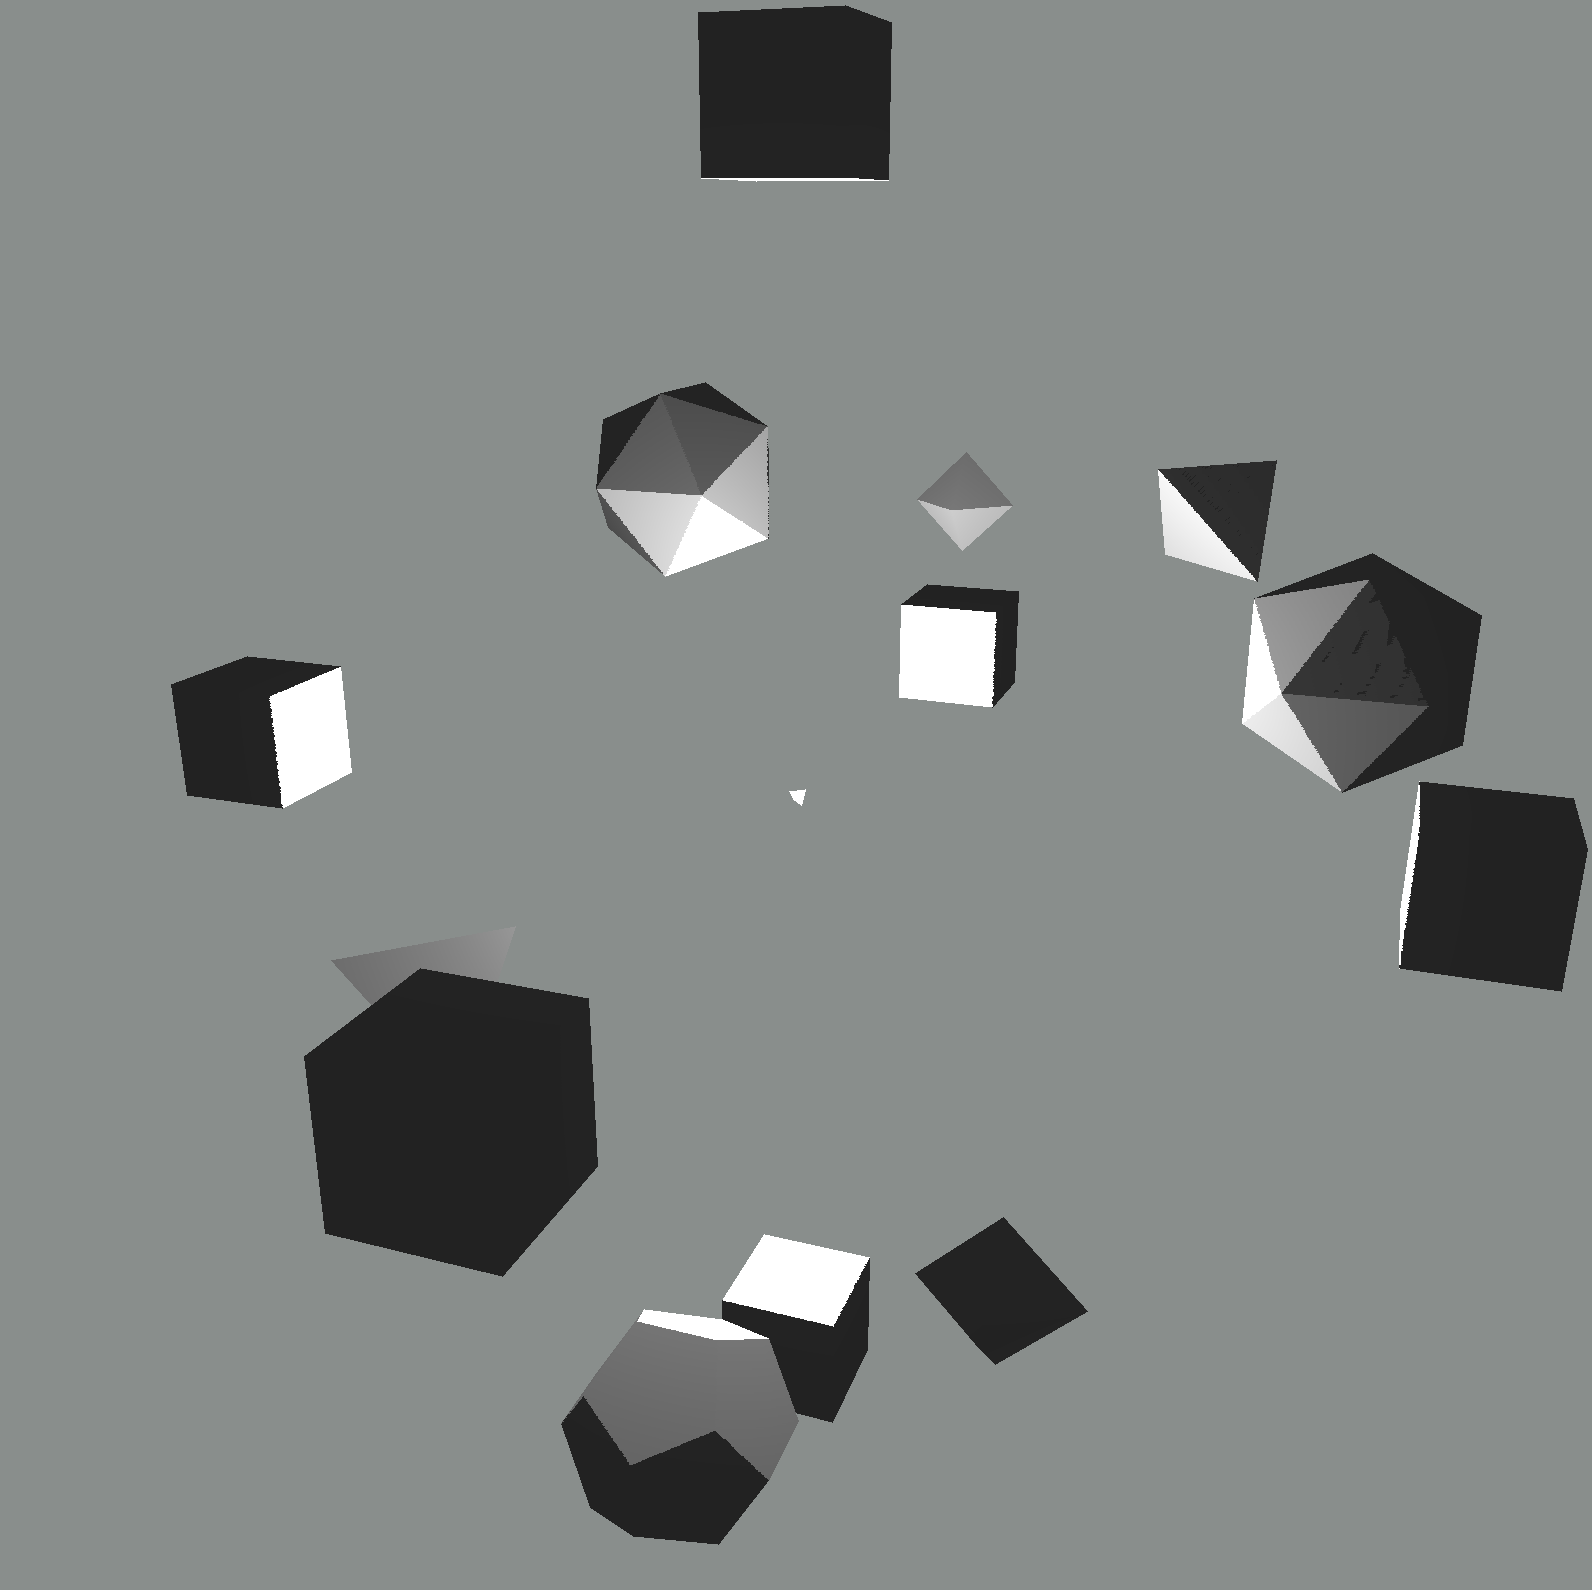
\includegraphics[width=0.3\textwidth]{rakurs1}
	\hfil
	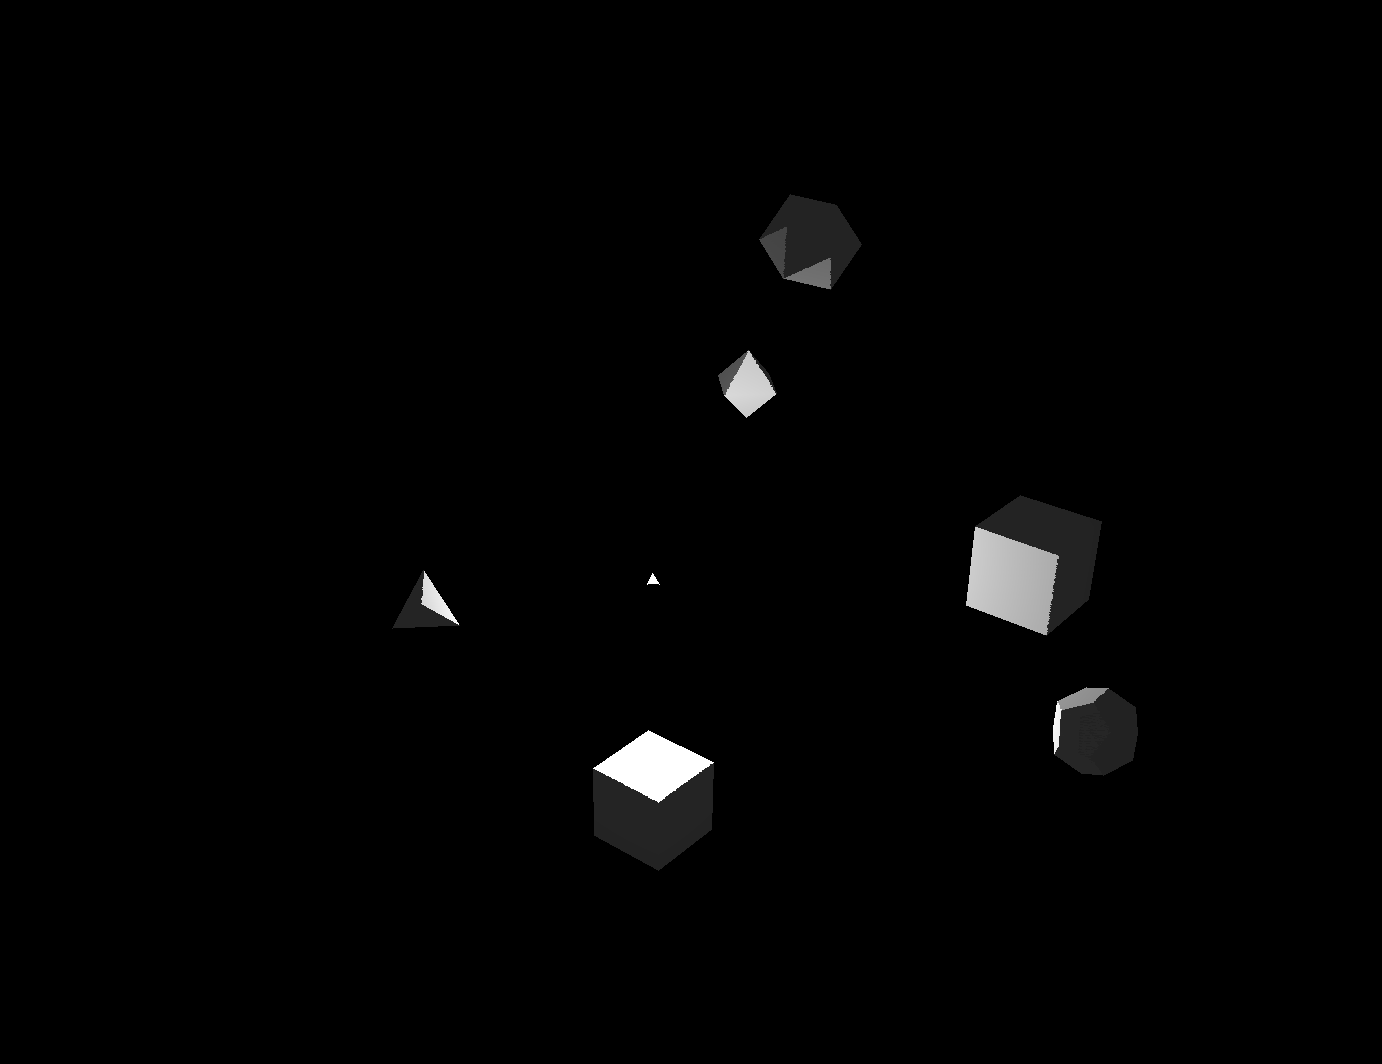
\includegraphics[width=0.3\textwidth]{rakurs2}
	\hfil
	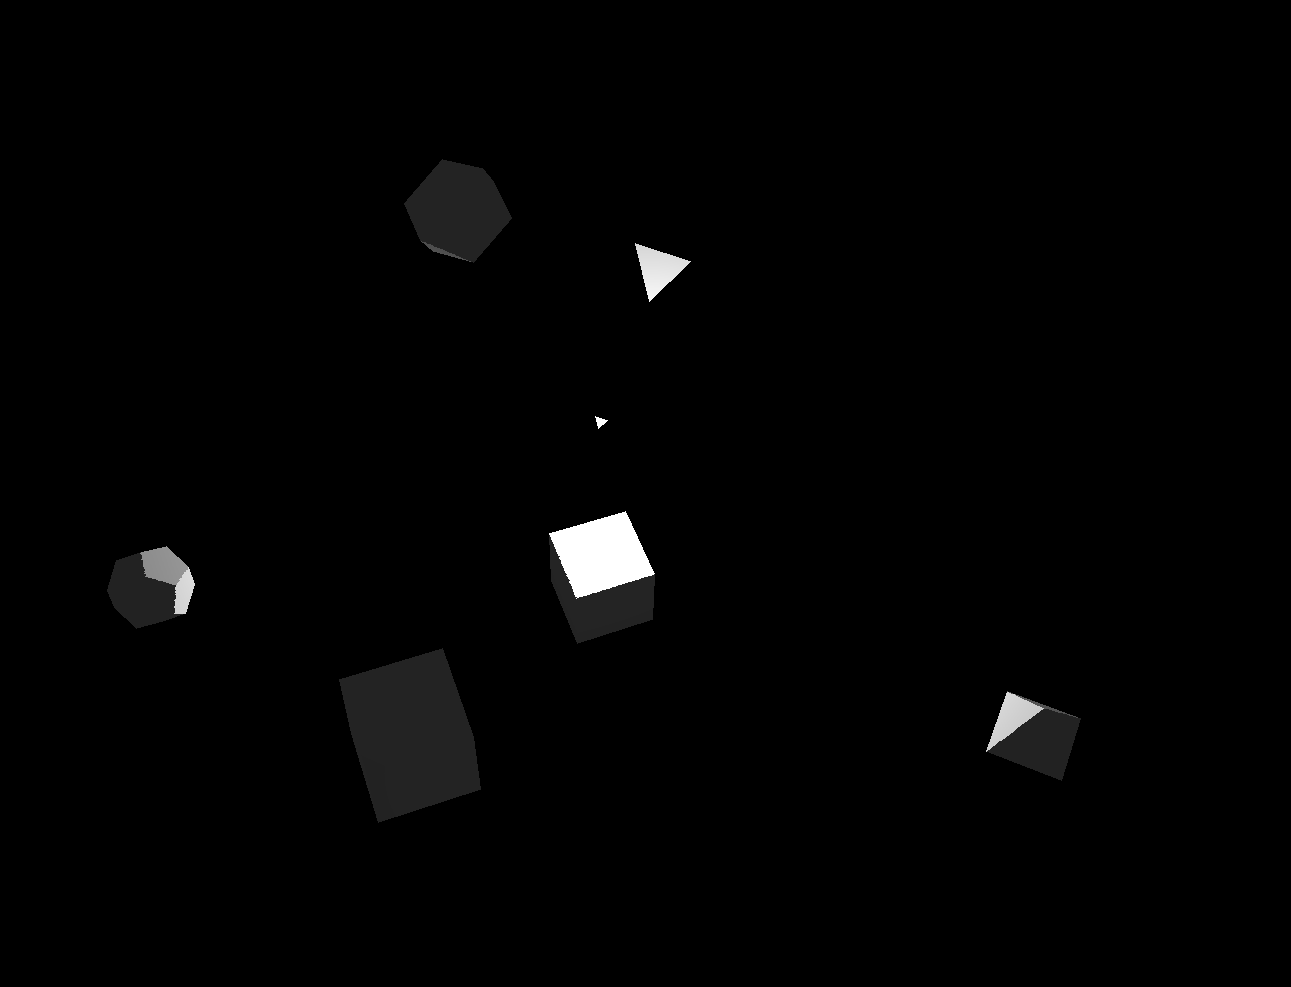
\includegraphics[width=0.3\textwidth]{rakurs3}
	\caption{Сцена с разных ракурсов.}
	\label{fig:racurs2}
\end{figure}

На рисунке~\ref{fig:shadow512} представлена сцена, на которой демонстрируются тени созданные алгоритмом теневых карт при разрешении буферов 512 на 512. На рисунке~\ref{fig:shadow2048} представлена  та же сцена, но при увеличенном разрешении -- 2048  на 2048. Как и ожидалось, во втором варианте тении имеют более гладкие края.

\begin{figure}[H]
	\centering
	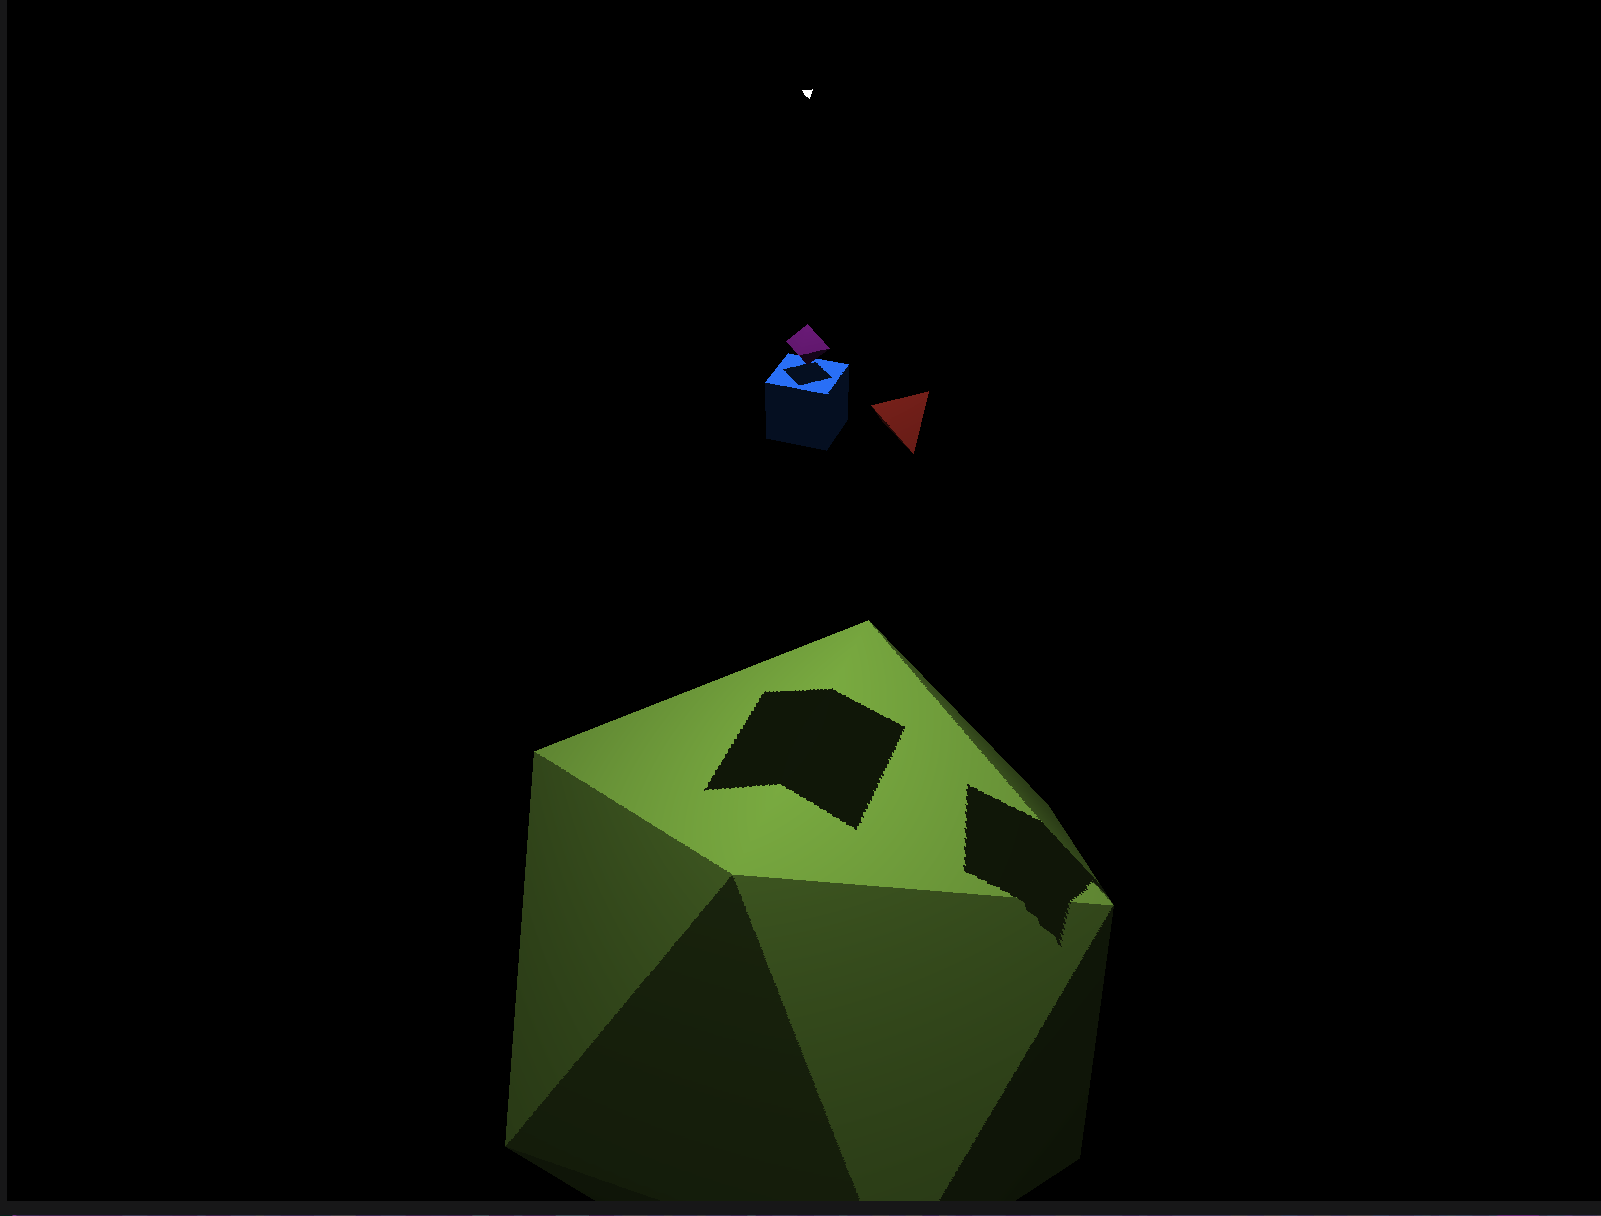
\includegraphics[width=0.7\textwidth]{shadow512}
	\caption{Тени созданные теневыми картами при разрешении 512x512.}
	\label{fig:shadow512}
\end{figure}


\begin{figure}[H]
	\centering
	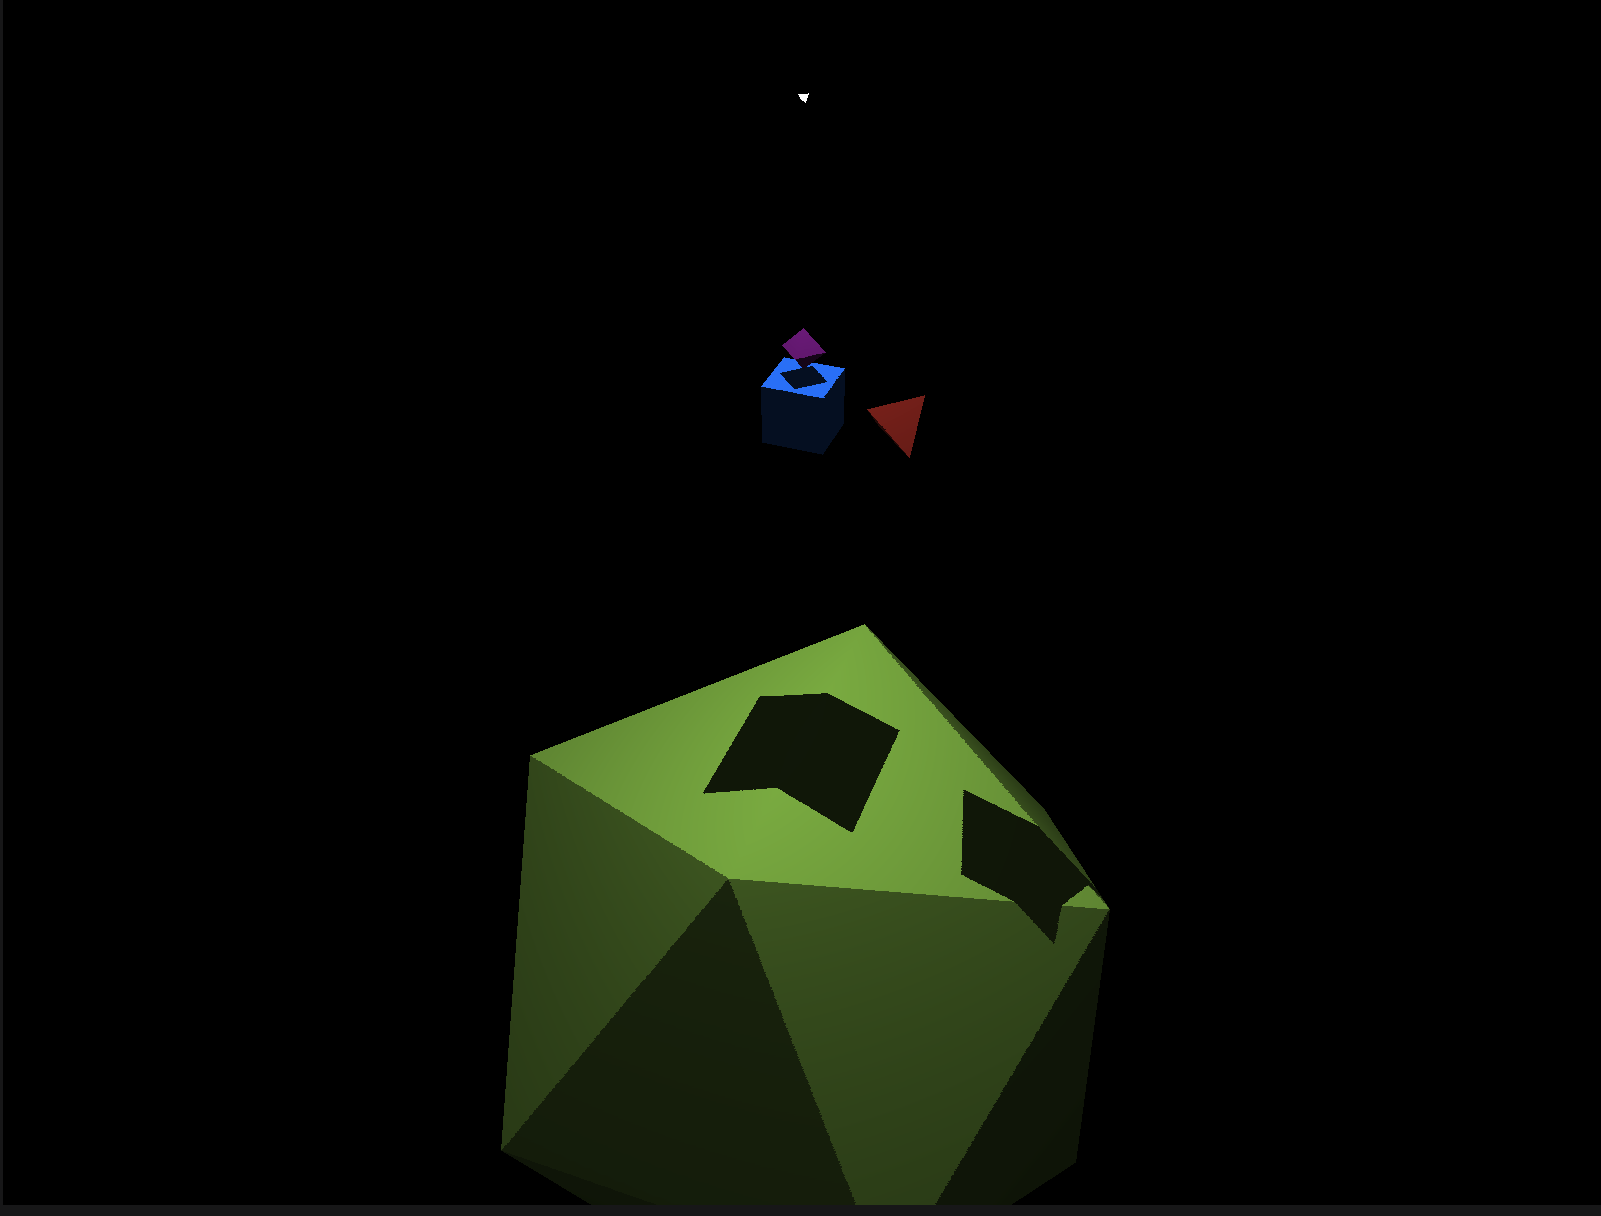
\includegraphics[width=0.7\textwidth]{shadow2048}
	\caption{Тени созданные теневыми картами при разрешении 2048x2048.}
	\label{fig:shadow2048}
\end{figure}

На рисунке~\ref{fig:sim} представлена сцена, полученная после расчётов задачи n тел в течении некоторого времени.

\begin{figure}[H]
	\centering
	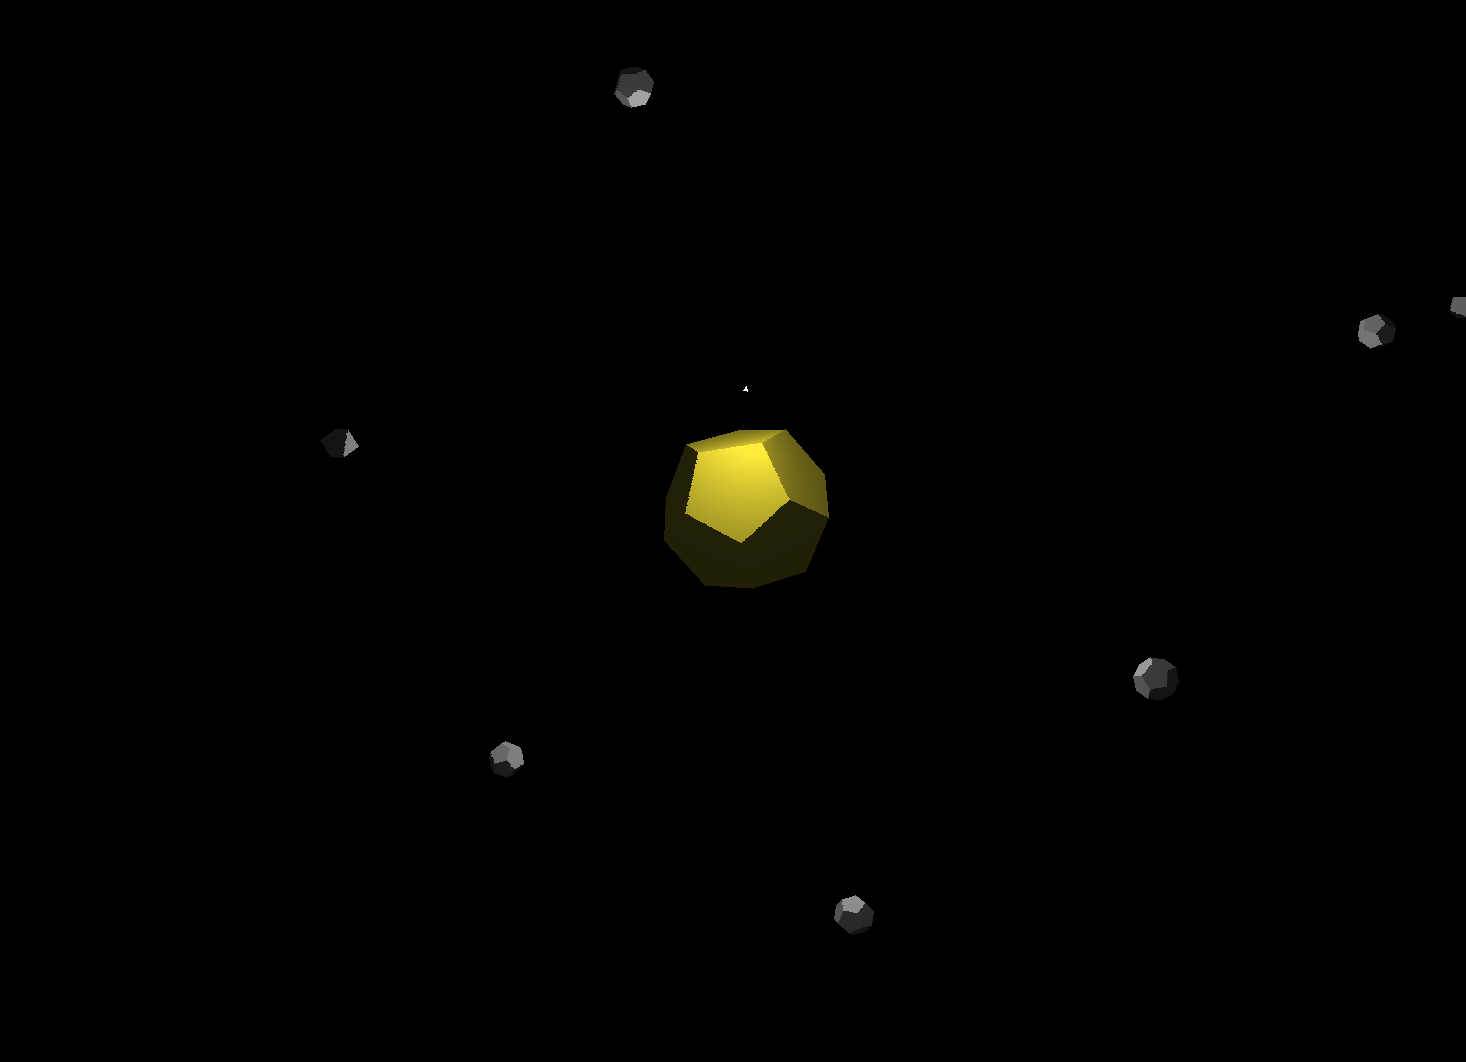
\includegraphics[width=0.5\textwidth]{central}
	\caption{Симуляция после некоторого времени после запуска.}
	\label{fig:sim}
\end{figure}


\section*{Вывод}

Было реализовано программное обеспечение с графическим интерфейсом для визуализации задачи n тел.

\clearpage
